\documentclass[printMode=false, declarePage=false]{ecnuthesis}
% 在printMode = false时,不会显示扫描版声明页,但printMode = true时,会空出一页以保证翻页正常
\ecnuSetup{
    info = {
        title = {深度学习中的梯度下降研究综述},
        %
        titleEN = {《问题驱动的算法设计》课程报告},
        %
        author = {张梓卫},
        %
        studentID = {10235101526},
        %
        department = {软件工程学院},
        %
        major = {软件工程},
        %
        supervisor = {蒲戈光},
        %
        year  = 2024,
        %
        month = 5,
        %
        day = 22,
        %
        graduationYear = 2027,
        %   若 graduationYear 字段为空,则内封面毕业届别为 year
        keywords = {梯度下降, 深度学习, 人工智能, 优化器, 大模型},
        %
        keywordsEN = {Gradient Descent, Deep Learning, Artificial Intelligence, Optimizer, Large Model},
    },
    style = {
        numbering = arabic,
        % 章节编号样式
        % 可用选项:
        %   numbering = arabic|alpha|chinese
        % 说明:
        %   arabic    使用数字进行编号 (即理科要求)
        %   alpha     使用字母进行编号 (即外文要求)
        %   chinese   使用汉字进行编号 (即文科要求)
        %   (默认选项为 arabic )
        %
        font = times,
        % 西文字体选择
        % 可用选项:
        %   font = lm|times|xits
        % 说明:
        %   lm        使用 TeX 自带的 Latin Modern 字体
        %   lm        使用 TeX 自带的 XITS 系列字体
        %   times     使用 Times 风格的西文字体
        %   (默认选项为 xits )
        %
        fontCJK = windows,
        % 中文字体选择
        % 可用选项:
        %   fontCJK = fandol|windows|mac
        % 说明:
        %   fandol    使用 TeX 自带的 fandol 字体
        %   windows   使用 Windows 系统内的字体 (中易)
        %   mac       使用 MacOS 系统内的字体
        %   (默认选项为 fandol )
        %
        logoResource = {./ECNULogo.png},
        % 封面插图数据源
        % 模版已自带, 位于 ./source/inner-cover(contains_font).eps
        % 默认值为空
        %
        % declarePageResource = {./source/declaration.pdf},
        % 扫描版声明页 PDF 文件
        % 若该值为空则生成模版预定义的声明页;否则将插入指定路径所对应的 PDF 文件
        % 默认值为空
        %
        bibResource = {./bib/thesis-ref.bib},
        % 参考文献数据源
        % 由于使用的是 biber + biblatex , 所以必须明确给出 .bib 后缀名
        %
    }
}

\usepackage{enumitem}
\usepackage{mwe}
\usepackage{zhlipsum} % 中文乱数文本
\usepackage{amsmath}
\usepackage{graphicx}
\usepackage{geometry}
\usepackage{booktabs} % 表格库
\usepackage{titlesec} % 标题库
\usepackage{fancyhdr} % 页眉页脚库
\usepackage{lastpage} % 页码数库
\usepackage{listings} % 代码块包
\usepackage{xcolor}
\usepackage[hidelinks]{hyperref}
\usepackage{tikz}
\usepackage{tikz-qtree}
\usepackage{float} % 浮动体环境
\usepackage{subcaption} % 子图包
\usepackage{pgfplots} % 绘图包
\usepackage{pgfplotstable} % 表格绘图包
\usepackage{caption}
\usepackage[backend=biber,style=numeric,sorting=none]{biblatex}

%———————————————定义颜色—————————————————%

\definecolor{mygreen}{rgb}{0,0.6,0}
\definecolor{mygray}{rgb}{0.5,0.5,0.5}
\definecolor{mymauve}{rgb}{0.58,0,0.82}

\date{} % 留空,以让编译时去除日期

%————————————设置页眉、页脚——————————————%

\pagestyle{fancy} % 设置 plain style 的属性

% 设置页眉

\fancyhead[LE,RO]{~\thepage~} % 在偶数页的左侧,奇数页的右侧显示页码
\renewcommand{\headrulewidth}{1.2pt} % 页眉与正文之间的水平线粗细

% 设置页脚:在每页的右下脚以斜体显示书名

\fancyfoot[RO,RE]{\it Review By \LaTeX} % 使用意大利斜体显示
\renewcommand{\footrulewidth}{0.5pt} % 页脚水平线宽度

% 设置页码:在底部居中显示页码

% \pagestyle{fancy}
% \fancyfoot[C]{\kaishu 第 \thepage 页 \ 共 \pageref{LastPage} 页} % LastPage 需要二次编译以获取总页数

%——————————————代码块设置———————————————%

\lstset {
    backgroundcolor=\color{white},   % 选择背景颜色;你必须添加 \usepackage{color} 或 \usepackage{xcolor}
    basicstyle=\footnotesize,        % 设置代码字体的大小
    breakatwhitespace=false,         % 设置是否只在空白处自动换行
    breaklines=true,                 % 设置自动换行
    captionpos=bl,                   % 设置标题位置为底部
    commentstyle=\color{mygreen},    % 注释样式
    deletekeywords={...},            % 如果你想从给定语言中删除关键词
    escapeinside={\%*}{*},           % 如果你想在代码中添加 LaTeX
    extendedchars=true,              % 允许使用非 ASCII 字符;仅适用于 8 位编码,不适用于 UTF-8
    frame=single,                    % 在代码周围添加框架
    keepspaces=true,                 % 保持文本中的空格,对于保持代码缩进有用(可能需要 columns=flexible)
    keywordstyle=\color{blue},       % 关键词样式
    % language=Python,               % 代码语言
    morekeywords={*,...},            % 如果你想向关键词集中添加更多关键词
    numbers=left,                    % 设置行号的位置;可能的值有(none, left, right)
    numbersep=5pt,                   % 行号与代码之间的距离
    numberstyle=\tiny\color{mygray}, % 行号的样式
    rulecolor=\color{black},         % 如果未设置,框架颜色可能会在非黑色文本(例如注释(此处为绿色))换行时更改
    showspaces=false,                % 在所有地方显示空格并添加特定下划线;它会覆盖 'showstringspaces'
    showstringspaces=false,          % 仅在字符串中显示空格
    showtabs=false,                  % 在字符串中显示制表符并添加特定下划线
    stepnumber=1,                    % 两个行号之间的步长。如果设置为 1,每行都会编号
    stringstyle=\color{orange},      % 字符串字面量样式
    tabsize=4,                       % 设置默认制表符大小为 4 个空格
    % title=Python Code              % 显示 \lstinputlisting 包含文件的文件名;也可以尝试使用 caption 替代 title    
}

% 注释掉的部分用于后续插入代码,参数可调整,格式如下:

% 1、直接插入
% \begin{lstlisting}[language = ? , title = { ? } ]
%       Your code here.
% \end{lstlisting}
% 注意,Title 不能有下划线,否则会报错。

% 2、文件插入
% \lstinputlisting[language = C , title = ?.c] {filename.c}

%———————————————字体设置————————————————%

% \setCJKmainfont{SimSun} % 设置正文罗马族的 CJK 字体
% \renewcommand{\normalsize}{\fontsize{12pt}{15pt}\selectfont} % 设置正文字号
\linespread{1.2}

%———————————————超链接设置——————————————%

\hypersetup{
    pdfstartview=FitH, % 设置PDF文档打开时的初始视图为页面宽度适应窗口宽度(即页面水平适应)
    CJKbookmarks=true, % 用对CJK(中文、日文、韩文)字符的书签支持,确保这些字符在书签中正确显示
    bookmarksnumbered=true, % 书签带有章节编号。这对有章节编号的文档很有用
    bookmarksopen=true, % 文档打开时,书签树是展开的,方便查看所有书签
    colorlinks, % 启用彩色链接。这样,链接在PDF中会显示为彩色,而不是默认的方框
    pdfborder=001, % 设置PDF文档中链接的边框样式。001 表示链接周围没有边框,仅在单击时显示一个矩形
    linkcolor=blue, % 设置文档内部链接(如目录中的章节链接)的颜色为蓝色
    anchorcolor=blue, % 设置锚点链接(即目标在同一文档内的链接)的颜色为蓝色
    citecolor=blue, % 设置引用(如文献引用)的颜色为蓝色
}

%——————————————导言区结束,进入正文部分———————————————%

\begin{document}

% 目录
    \tableofcontents

% 声明前置部分开始, 页码设置为大写罗马数字
    \frontmatter

    \begin{abstract}
        梯度下降是许多机器学习算法的基石,也是最受欢迎的优化算法之一。
        梯度下降的原理是通过迭代地调整参数来最小化损失函数。
        它是深度学习和优化领域的基本算法,对于模型的训练和微调至关重要。
        该迭代方法通过沿最陡下降方向移动来最小化函数,该方向由负梯度确定。
        梯度下降的重要性跨越了多个领域,从简单的线性回归模型到复杂的深度神经网络。
        本篇文献综述旨在全面概述梯度下降,追踪其历史发展,解释其基本概念,探索其各种增强,并检查其在机器学习中的应用。
        通过深入探讨理论基础和实际考虑,本综述旨在提供对梯度下降及其在人工智能领域持久影响的全面理解。
        旨在整理梯度下降在人工智能领域的发展脉络,为研究者提供一些文献参考和未来工作展望。
    \end{abstract}

    \begin{abstractEN}
        Gradient descent is the cornerstone of many machine learning algorithms and one of the most popular optimization algorithms.
        The principle of gradient descent is to minimize the loss function by iteratively adjusting parameters.
        This article aims to provide a comprehensive overview of gradient descent and its various extensions, covering theoretical aspects, practical applications, and recent developments.
        It is a fundamental algorithm in the field of machine learning and optimization, and is crucial for model training and fine-tuning.
        This iterative method minimizes the function by moving along the steepest descent direction, which is determined by a negative gradient.
        The importance of gradient descent spans multiple fields, from simple linear regression models to complex deep neural networks.
        This literature review aims to provide a comprehensive overview of gradient descent, track its historical development,
        explain its basic concepts, explore its various enhancements, 
        and examine its applications in machine learning.
        Through in-depth exploration of theoretical foundations and practical considerations, 
        this review aims to provide a comprehensive understanding of gradient descent and its persistent 
        impact in the field of artificial intelligence.
        The aim is to sort out the development of gradient descent in the field of artificial intelligence, and provide some literature references and future work prospects for researchers.
    \end{abstractEN}

% 声明正文部分开始, 页码设置为阿拉伯数字
    \mainmatter

    \chapter{引言}


    \section{深度学习应用中的一个故事或引例}

    数学家$Augustin-Louis\ Cauchy$在$1847$年首次发明了梯度下降法\cite{lemarechal2012cauchy},
    这是由于需要解决天文学中出现的“大型”二次问题($6$个变量)
    今天,这种方法被用来轻松地解决具有数千个变量的问题.用于解决天文学计算和估计恒星轨道.\cite{coursera2024gradientdescent}
    本文主要专注于了解它在优化机器学习算法中所扮演的角色,以及引申出其他的一些相关概念.

    \section{早期数学基础}

    在深度学习算法中, 梯度下降 ($Gradient\ Descent$) 是一种用于优化和训练机器学习模型的迭代算法.
    它通过逐步调整模型参数以最小化损失函数 (即模型预测与实际值之间的误差), 找到模型参数的最优值,
    从而找到问题的一种解决方案.

    梯度下降法的基本思想源于微积分中的梯度概念.
    梯度是多变量函数的方向导数, 表示函数在某点的最大上升方向.
    19 世纪的数学家如卡尔·弗里德里希·高斯 ($Carl\ Friedrich\ Gauss$) 和奥古斯丁·路易斯·柯西 ($Augustin-Louis\ Cauchy$) 在优化问题中已经使用了类似的思想.

    \section{历史的更迭}

    梯度下降法的提出和发展有着深刻的历史背景和原因。理解这些背景有助于我更好地把握这一数学概念和方法的意义及其应用。

    \subsection{早期优化问题的研究}
    在19世纪中叶, 随着微积分和变分法的发展, 数学家们开始关注如何求解复杂函数的极值问题。考克斯($Augustin-Louis\ Cauchy$)于$1847$年提出了梯度下降法, 作为求解这些问题的一种有效方法。这一时期的研究主要集中在理论层面, 探讨了函数极值的性质及其计算方法。

    \subsection{计算机的发展}
    20世纪中叶, 随着电子计算机的发明和发展, 数值计算成为可能。梯度下降法作为一种数值优化算法, 逐渐在计算机科学中得到应用。计算机的高速计算能力使得梯度下降法能够处理大规模的优化问题, 推动了该方法的实际应用和进一步发展。

    \subsection{机器学习的兴起}
    20世纪末至21世纪初, 机器学习迅速发展成为一门重要的学科。梯度下降法作为机器学习模型训练中的核心算法之一, 得到了广泛应用。尤其在神经网络和深度学习领域, 梯度下降法被用来优化模型参数, 从而提高模型的性能。这一时期, 各种梯度下降法的变种(如随机梯度下降, 动量梯度下降, 自适应学习率方法等)也相继被提出和应用, 进一步丰富了梯度下降法的理论和实践。

    \subsection{大数据和人工智能的推动}
    进入21世纪, 大数据和人工智能的蓬勃发展对梯度下降法提出了新的挑战和需求。面对海量数据和复杂模型, 传统的梯度下降法在计算效率和收敛性方面遇到了一些问题。为此, 研究者们提出了一系列改进和优化策略, 如分布式梯度下降, 并行计算等, 以适应大规模数据处理的需求。

    \subsection{多学科交叉的影响}
    梯度下降法不仅在数学和计算机科学中发挥重要作用, 还与物理学, 工程学, 经济学等多个学科紧密相关。不同领域的问题和需求推动了梯度下降法的不断发展和完善, 使其在理论和应用上都取得了显著的进步。
    它的提出和发展有着深厚的历史背景和多方面的推动因素。从早期的理论研究到现代的广泛应用, 梯度下降法不断演进, 成为解决优化问题的重要工具。

    \paragraph{高斯牛顿法}

    高斯-牛顿法用于求解非线性最小二乘问题, 目标是最小化残差平方和.\cite{lai2017solving}
    算法的基本步骤包括:
    1.
    初始猜测参数值.
    2.
    计算残差和雅可比矩阵.
    3.
    使用线性近似来更新参数值.
    4.
    迭代上述步骤直到收敛.
    高斯-牛顿法的更新公式为:
    \begin{equation}
        \mathbf{x}_{k+1} = \mathbf{x}_k + \Delta \mathbf{x}_k
    \end{equation}
    其中,\(\Delta \mathbf{x}_k\) 是在第 \(k\) 次迭代时参数更新的增量,可以通过解下列线性方程组得到:
    \begin{equation}
        \mathbf{J}^T \mathbf{J} \Delta \mathbf{x}_k = -\mathbf{J}^T \mathbf{f}(\mathbf{x}_k)
    \end{equation}

    这里:
    - \(\mathbf{J}\) 是目标函数关于参数的雅可比矩阵($Jacobian\ Matrix$)。
    - \(\mathbf{f}(\mathbf{x}_k)\) 是在第 \(k\) 次迭代时目标函数的残差向量。
    - \(\mathbf{x}_k\) 是在第 \(k\) 次迭代时的参数估计值。
    - \(\mathbf{J}^T\) 是雅可比矩阵的转置。

    高斯通过引入雅可比矩阵和线性近似的思想,为后来的梯度下降法及其变体提供了重要的理论基础.\cite{schraudolph2002fast}
    他的方法在求解非线性优化问题中发挥了重要作用。

    \paragraph{柯西梯度法}

    柯西在$1847$年提出了一种求解非线性方程的迭代方法,这种方法后来被称为 "柯西梯度法"  ($Cauchy\ Gradient\ 
    Method$) ,也是梯度下降法的早期形式。\cite{hassan2009new}

    柯西梯度法的基本思想:
    柯西梯度法旨在找到一个函数的局部极小值,通过沿负梯度方向进行迭代来逐步逼近极小值点。

    高斯和柯西的工作对优化理论的发展具有深远影响。
    高斯通过高斯-牛顿法引入了雅可比矩阵和线性近似的概念,
    为非线性优化问题提供了有效的解决方案。
    而柯西通过柯西梯度法提出了沿梯度方向进行迭代的方法,
    为梯度下降法奠定了基础。

    \chapter{梯度下降法的主要内容}

    梯度下降法($Gradient\ Descent$)是一种优化算法,主要用于寻找使函数值最小化的变量值。其核心思想是沿着函数梯度的反方向迭代,以逐步逼近函数的局部最小值。梯度下降法在机器学习和深度学习中被广泛应用于模型训练过程中的参数优化。

    求解模型 ($1$) 的梯度下降算法包括全梯度下降 ($Full\ gradient\ descent$,$FGD$) \cite{becker1988improving}、随机梯度下降 ($SGD$) \cite{nesterov2013gradient} 和小批量梯度下降 (Mini-batch gradient descent, Mini-batch) \cite{hinton2012neural, li2014efficient}。

    $FGD$ 以目标函数的全梯度 (即全部子函数数梯度的平均值)迭代求解,参数更新式为
    \begin{equation}
    \theta_{t+1} = \theta_t - \frac{\alpha_t}{n} \sum_{i=1}^n \nabla f_i(\theta_t)
    \end{equation}

    其中,$\alpha_t$ 为第 $t$ 轮迭代的学习率,用于调整参数更新的幅度。为防止学习率过大而造成振荡,常将其设置为一个较小的常量或递减的序列。当目标函数 $J$ 为凸函数时,FGD 可取得收敛速度为 $O(1/t)$ 的次线性收敛速度,

    与 $FGD$ 相比,随机梯度下降 ($SGD$) 仅随机抽取一个样本或子函数来计算其梯度,并以此梯度为全局梯度的估计值。$SGD$ 的参数更新式为
    \begin{equation}
    \theta_{t+1} = \theta_t - \alpha_t \nabla f_{i_t}(\theta_t)
    \end{equation}

    其中,$i_t \in \{1, 2, \ldots, n\}$ 表示第 $t$ 轮迭代中按均匀分布随机抽取的样本或子函数。由于每次迭代只需计算一个样本的梯度,迭代成本较小,但由于更新方向的随机性,迭代路径会有较大波动。为了实用中的高效性,使用 SGD 常难以滑落到最优解的更新方向逼近最优。

    对于 $FGD$ 和 $SGD$,在每次迭代中,$FGD$ 都能改进目标函数,而 $SGD$ 则在振荡中收敛至最优解。\cite{史加荣2021随机梯度下降算法研究进展}


    \section{梯度下降法的基本思想}
    梯度下降法的目标是找到目标函数 \( f(\mathbf{x}) \) 的极小值点。具体来说,假设我有一个可微的目标函数 \( f(\mathbf{x}) \),其中 \( \mathbf{x} \) 是变量向量。梯度下降法通过以下更新规则迭代地调整变量 \( \mathbf{x} \):
    \begin{equation}
        \mathbf{x}_{k+1} = \mathbf{x}_k - \eta \nabla f(\mathbf{x}_k)
    \end{equation}
    其中,\( \mathbf{x}_k \) 表示第 \( k \) 次迭代的变量值,\( \eta \) 是学习率(步长),\( \nabla f(\mathbf{x}_k) \) 是函数 \( f \) 在 \( \mathbf{x}_k \) 处的梯度。

    \subsection{梯度的定义}
    梯度(Gradient)是由多变量函数的偏导数组成的向量。对于函数 \( f(\mathbf{x}) \),其梯度定义为:
    \begin{equation}
        \nabla f(\mathbf{x}) = \left( \frac{\partial f}{\partial x_1}, \frac{\partial f}{\partial x_2}, \ldots, \frac{\partial f}{\partial x_n} \right)^T
    \end{equation}
    梯度指向函数值增长最快的方向,因此,沿梯度的反方向移动可以使函数值减小。

    \subsection{梯度下降法的提出与应用}
    梯度下降法的基本形式可以追溯到$19$世纪,由考克斯($Augustin-Louis\ Cauchy$)于$1847$年首次提出。此后,梯度下降法被不断发展和完善,成为数值优化的重要工具。

    在机器学习中,梯度下降法被用来最小化损失函数,从而优化模型参数。例如,在线性回归中,梯度下降法用于最小化均方误差;在神经网络中,梯度下降法用于最小化交叉熵损失或其他损失函数。

    \subsection{学习率的选择}
    学习率 \( \eta \) 是梯度下降法中的一个重要参数,其值的选择对算法的收敛性和收敛速度有显著影响。
    如果学习率过大,算法可能会在最小值附近震荡或发散;
    如果学习率过小,算法收敛速度会非常慢。
    常用的方法是通过交叉验证或学习率调度策略来选择合适的学习率。\cite{yang2020auto}
    在学习过程中,我发现了一个网站,于是我选择它(\href{https://playground.tensorflow.org/}{$TensorFlow\ Playground$})来直观地展示不同学习率对梯度下降法的影响。
    
    \begin{figure}[htbp]
        \centering
        \begin{subfigure}[b]{0.3\textwidth}
            \centering
            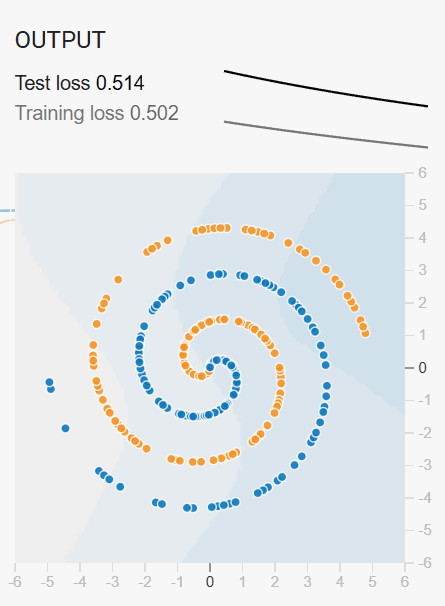
\includegraphics[width=\textwidth]{too-slow-000001.png}
            \caption{学习率过低导致速度过慢}
            \label{fig:step021}
        \end{subfigure}
        \hfill
        \begin{subfigure}[b]{0.3\textwidth}
            \centering
            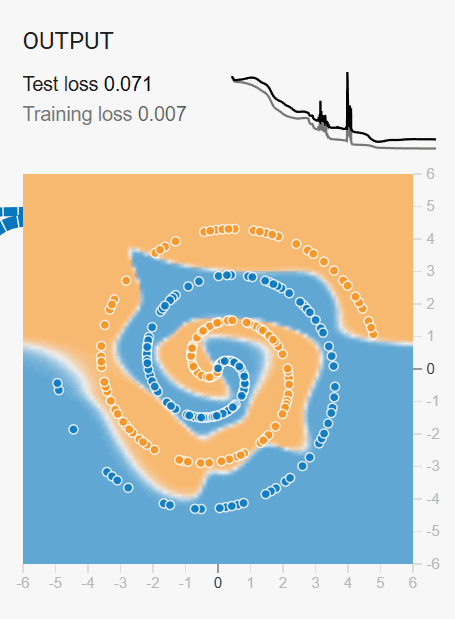
\includegraphics[width=\textwidth]{medium-003.png}
            \caption{学习率适中}
            \label{fig:step086}
        \end{subfigure}
        \hfill
        \begin{subfigure}[b]{0.3\textwidth}
            \centering
            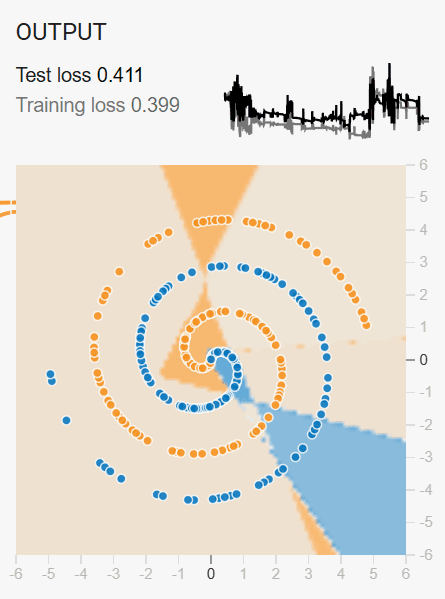
\includegraphics[width=\textwidth]{too-fast-1.png}
            \caption{学习率过大导致损失函数抖动}
            \label{fig:another}
        \end{subfigure}
        \caption{学习率的选择对输出结果的影响}
        \label{fig:comparison}
    \end{figure}

    \begin{figure}[H]
        \centering
        \begin{tikzpicture}
            \begin{axis}[
                width=\textwidth,
                height=0.3\textwidth,
                xlabel={迭代次数},
                ylabel={损失函数值},
                legend pos=north east,
                grid=major,
                xmin=0, xmax=10,
                ymin=0, ymax=1,
                legend style={font=\small}
            ]
            \addplot[blue, thick] table {
                0 1
                1 0.8
                2 0.6
                3 0.5
                4 0.4
                5 0.35
                6 0.3
                7 0.28
                8 0.26
                9 0.25
                10 0.24
            };
            \addlegendentry{较小的学习率}
            
            \addplot[red, thick] table {
                0 1
                1 0.7
                2 0.5
                3 0.4
                4 0.35
                5 0.3
                6 0.28
                7 0.26
                8 0.24
                9 0.23
                10 0.22
            };
            \addlegendentry{较大的学习率}
            
            \addplot[orange, thick] table {
                0 1
                1 0.85
                2 0.75
                3 0.7
                4 0.68
                5 0.67
                6 0.68
                7 0.7
                8 0.75
                9 0.85
                10 1
            };
            \addlegendentry{极大的学习率}
            
            \addplot[green, thick] table {
                0 1
                1 0.6
                2 0.4
                3 0.3
                4 0.25
                5 0.22
                6 0.2
                7 0.19
                8 0.18
                9 0.17
                10 0.16
            };
            \addlegendentry{适当的学习率}
            \end{axis}
        \end{tikzpicture}
        \caption{学习率对优化过程的影响}
        \label{fig:learning_rates}
    \end{figure}
    
    \begin{figure}[H]
        \centering
        \begin{tikzpicture}
            \begin{semilogyaxis}[
                width=\textwidth,
                height=0.3\textwidth,
                xlabel={全局迭代次数},
                ylabel={学习率},
                legend pos=south west,
                grid=major,
                xmin=0, xmax=15,
                ymin=1e-6, ymax=1e-2,
                legend style={font=\small}
            ]
            \addplot[black, thick] table {
                0 1e-2
                1 3e-3
                2 1e-3
                3 6e-4
                4 4e-4
                5 3e-4
                6 2.5e-4
                7 2e-4
                8 1.8e-4
                9 1.6e-4
                10 1.5e-4
                11 1.4e-4
                12 1.3e-4
                13 1.2e-4
                14 1.1e-4
                15 1e-4
            };
            \addlegendentry{分量1}
            
            \addplot[red, thick] table {
                0 1e-2
                1 4e-3
                2 1.5e-3
                3 9e-4
                4 6e-4
                5 5e-4
                6 4e-4
                7 3.5e-4
                8 3e-4
                9 2.7e-4
                10 2.5e-4
                11 2.3e-4
                12 2.1e-4
                13 2e-4
                14 1.9e-4
                15 1.8e-4
            };
            \addlegendentry{分量2}
            
            \addplot[blue, thick] table {
                0 1e-2
                1 2e-3
                2 1e-3
                3 8e-4
                4 7e-4
                5 6e-4
                6 5.5e-4
                7 5e-4
                8 4.5e-4
                9 4.2e-4
                10 4e-4
                11 3.8e-4
                12 3.6e-4
                13 3.5e-4
                14 3.4e-4
                15 3.3e-4
            };
            \addlegendentry{分量3}

            \end{semilogyaxis}
        \end{tikzpicture}
        \caption{Adagrad的学习率变化示意图}
        \label{fig:adagrad_learning_rates}
    \end{figure}

    \subsection{梯度下降法的变种}
    随着梯度下降法在实践中的广泛应用,出现了许多变种算法,以解决其原始形式的一些缺陷。这些变种包括:
    \begin{itemize}
        \item 随机梯度下降($Stochastic\ Gradient\ Descent,\ SGD$):每次迭代仅使用一个样本来更新梯度,适用于大规模数据集。
        \item 小批量梯度下降($Mini-batch\ Gradient\ Descent$):每次迭代使用一小批样本来更新梯度,兼顾了批量梯度下降和随机梯度下降的优点。
        \item 动量梯度下降($Momentum\ Gradient\ Descent$):引入动量项,减少迭代过程中的震荡,加速收敛。
        \item 自适应学习率方法(如$AdaGrad,\ RMSprop,\ Adam$):根据梯度信息动态调整学习率,提高收敛效率。
    \end{itemize}

    但梯度下降法的核心是优化问题,即在一定条件下找到函数的极小值。优化思维贯穿于整个算法中,包括目标函数的构建,学习率的选择,以及收敛性的分析。
    梯度下降法依赖于函数的导数和梯度信息,这些都是微积分的基本概念。通过计算梯度并沿梯度的反方向移动,我能够逐步逼近函数的极小值点,这是微积分在优化问题中的一种具体应用。
    
    \subsection{迭代思维}
    梯度下降法是一种迭代算法,通过反复更新变量的值来逼近最优解。\cite{haji2021comparison}
    迭代思维要求我在每一步更新中都要考虑当前的梯度信息,并合理调整步长,以确保算法的收敛性和效率。
    如下所示:我使用网站:
    \href{https://fa.bianp.net/teaching/2018/COMP-652/gradient_descent.html}{Fabianp}来控制调整步长,以便更好地理解梯度下降法的工作原理。
    
    \begin{figure} [H]
        \centering
        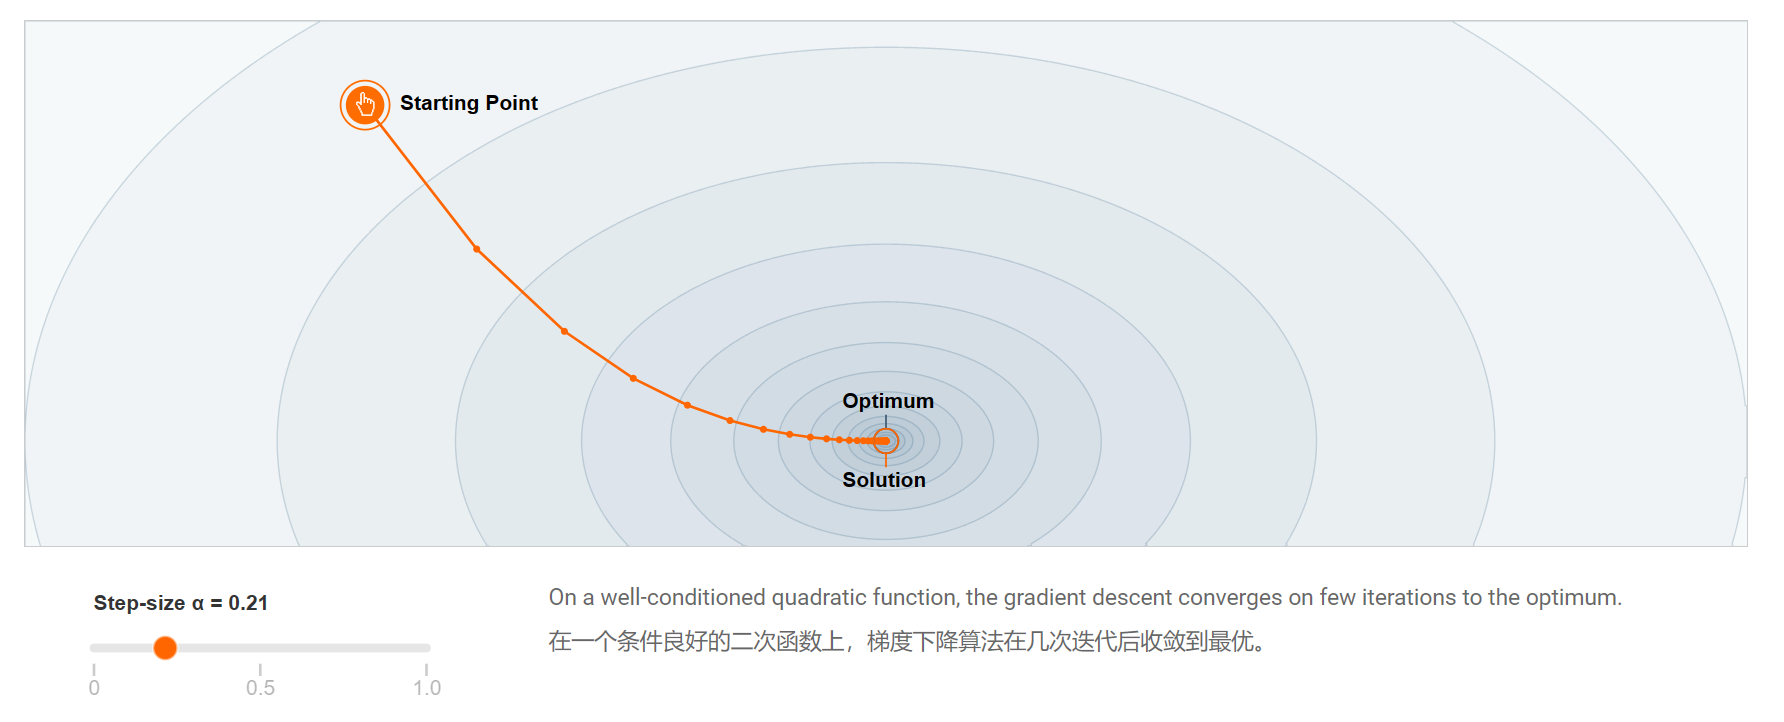
\includegraphics[width=0.9\textwidth]{Step021.png}
        \caption{Step-Size:0.21}
        \label{fig:gradient-descent}
    \end{figure}

    \begin{figure} [H]
        \centering
        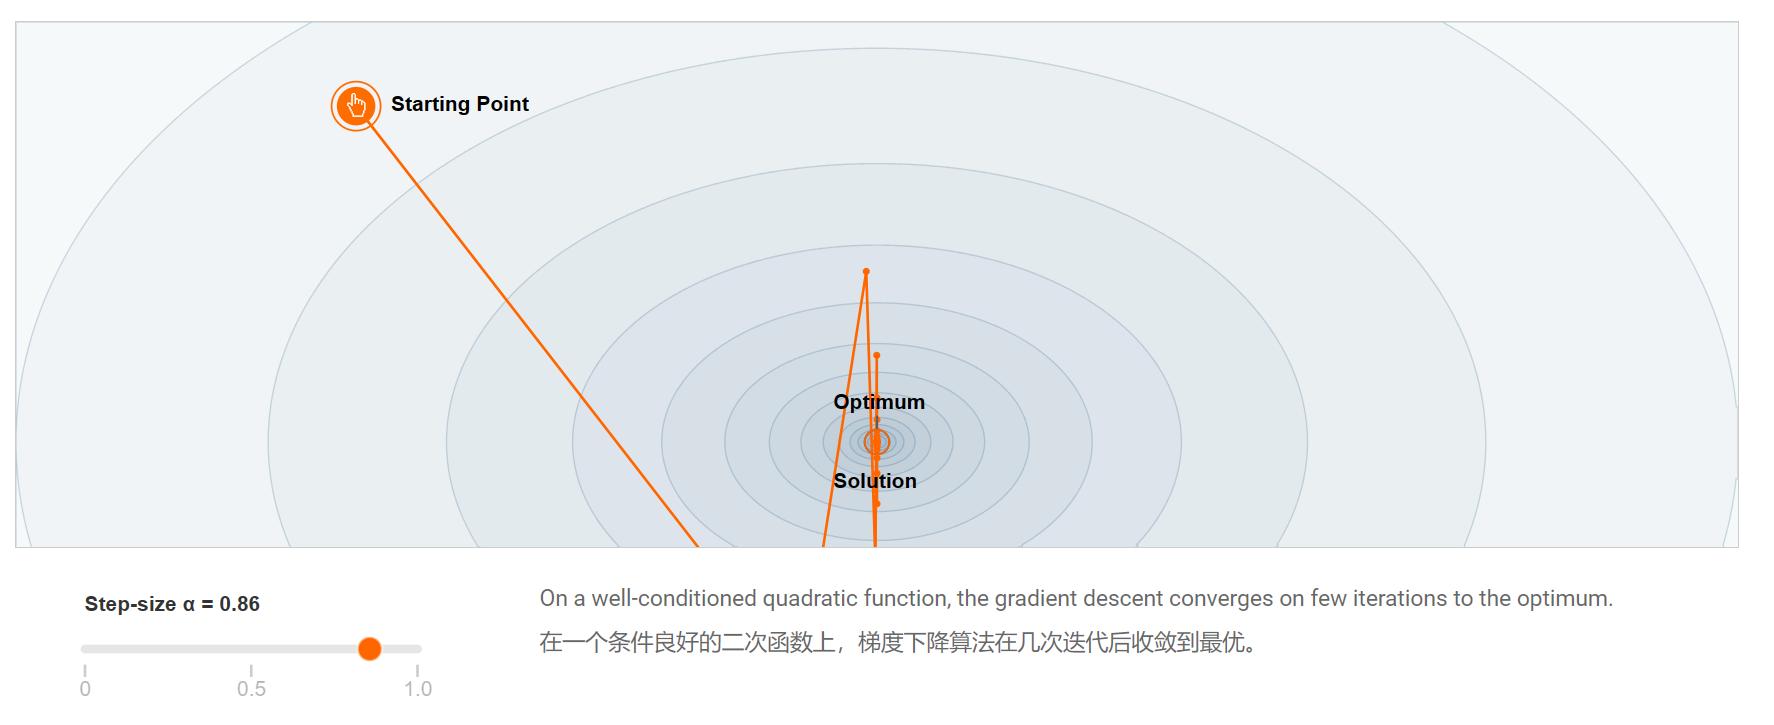
\includegraphics[width=0.9\textwidth]{Step086.png}
        \caption{Step-Size:0.86}
        \label{fig:gradient-descent}
    \end{figure}

    在后图中,步长较大($0.86$),算法在每次更新时跨越的距离较大,容易在损失函数的不同区域之间来回振荡,甚至可能偏离最优解。\cite{becker1988improving}
    图中可以看到,迭代路径出现了大幅度的跳动,且在最优解附近有明显的振荡,虽然最终也收敛到最优解,但收敛过程不稳定。
    因此,后人们使用了许多算法,步长的选择需要在过小和过大之间找到平衡,以确保收敛速度和稳定性。
    一般可以通过实验或使用自适应步长算法(如$AdaGrad$、$RMSprop$、$Adam$等)来优化步长选择。

    这一部分见后文中介绍的内容。

    \subsection{数值分析思维}
    在实际应用中, 梯度下降法需要处理各种数值问题, 如梯度计算的精度, 学习率的选择, 以及算法的收敛速度等。数值分析思维帮助我在实现和应用梯度下降法时, 解决这些实际问题, 提高算法的稳定性和效率。

    随着时间的推移和技术的发展, 梯度下降法不断地被改进和发展, 以满足不同应用场景的需求。

    \subsection{随机梯度下降实例($SGD$)}
    传统的梯度下降法每次迭代都会使用整个数据集计算梯度, 对于大规模数据集, 这种方法计算量大且效率低。随机梯度下降法($SGD$)通过在每次迭代中随机选取一个样本来更新梯度, 大大提高了计算效率。

    在研究$SGD$随机梯度下降算法时,我通过研究最典型的$SGD$代码实现,来更好地理解$SGD$的工作原理。

    \begin{lstlisting}[language = python, title = {$SGD\ Algorithm$}]
        import torch
        from torch import nn, optim
        
        # 定义一个简单的线性模型
        model = nn.Linear(2, 1)  # 输入2个特征, 输出1个值
        
        # 假设有输入数据和标签
        inputs = torch.randn(100, 2)  # 100个样本, 每个样本2个特征
        labels = torch.randn(100, 1)  # 100个样本, 每个样本1个标签
        
        # 创建优化器, 指定要更新的模型参数
        optimizer = optim.SGD(model.parameters(), lr=0.01)  # 学习率为0.01
        outputs = model(inputs)                        # 前向传播
        loss = nn.MSELoss()(outputs, labels)           # 损失函数
        loss.backward()                                # 反向传播并计算梯度
        optimizer.step()                               # 使用优化器更新参数
        optimizer.zero_grad()                          # 清除梯度(防止梯度累积)
    \end{lstlisting}

    在运行代码时, 我使用了zero\_grad来清除梯度, 为何要进行最后的这一步操作呢?
    在学习的过程中,
    我了解到:

    ``梯度累积''指: 多个批次或样本上计算梯度时, 将梯度相加累积的情况。\cite{lin2017deep}
    梯度累积会导致参数更新步骤推迟,
    尤其是在训练过程中使用较大的学习率时。
    较大的梯度可能导致模型参数跳跃到不良的局部最小值或发散的情况。
    因为只有在清除梯度后, 才能执行参数更新。
    这可能导致梯度更新的频率降低, 从而延缓模型的收敛速度。

    那么, 没有$optimizer.zero\_grad()$会发生什么呢?

    为了可视化相关的结果,
    我学习使用了$matplotlib$库来体现两者的差别。
    $Python$代码如下所示:

    \begin{lstlisting} [language = python, title = {Visualization} ]
        import torch
        from torch import nn, optim
        import matplotlib.pyplot as plt

        # 定义一个简单的线性模型
        model1 = nn.Linear(2, 1)  # 模型1
        model2 = nn.Linear(2, 1)  # 模型2

        # 假设有输入数据和标签
        inputs = torch.randn(100, 2)  # 10个样本,每个样本2个特征
        labels = torch.randn(100, 1)  # 10个样本,每个样本1个标签

        # 创建优化器
        optimizer1 = optim.SGD(model1.parameters(), lr=0.01)
        optimizer2 = optim.SGD(model2.parameters(), lr=0.01)

        # 用于记录损失
        losses_with_clear_grad = []
        losses_without_clear_grad = []

        # 训练100个步骤,清除梯度的情况
        for step in range(100):
            outputs = model1(inputs)
            loss = nn.MSELoss()(outputs, labels)
            losses_with_clear_grad.append(loss.item())

            optimizer1.zero_grad()  # 清除梯度
            loss.backward()
            optimizer1.step()

        # 训练100个步骤,不清除梯度的情况
        for step in range(100):
            outputs = model2(inputs)
            loss = nn.MSELoss()(outputs, labels)
            losses_without_clear_grad.append(loss.item())

            # 这里没有调用 zero_grad()
            loss.backward()
            optimizer2.step()

        # 可视化对比
        plt.plot(range(100), losses_with_clear_grad, marker='o', label='With Clear Gradients')
        plt.plot(range(100), losses_without_clear_grad, marker='x', label='Without Clear Gradients')
        plt.xlabel('Step')
        plt.ylabel('Loss')
        plt.title('Loss during Training')
        plt.legend()
        plt.show()
    \end{lstlisting}

    含有梯度清除和不含梯度清除时, 两者的差别如下图所示:

    \begin{figure} [H]
        \centering
        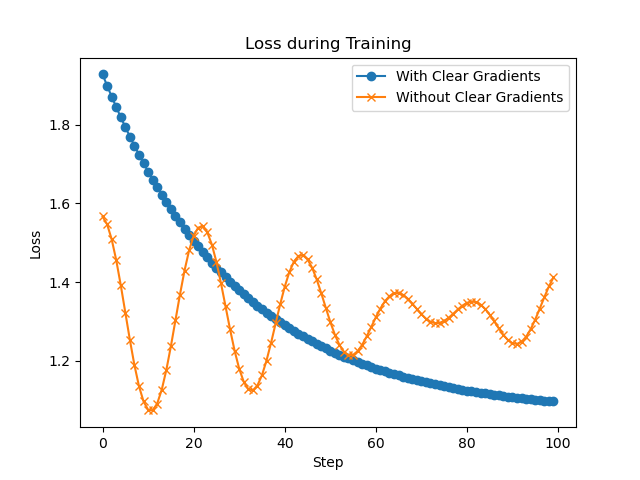
\includegraphics[width=0.6\textwidth]{../lectures/img/clear-gradients.png}
        \caption{梯度清除与不清除的损失对比}
    \end{figure}

    在每个批次或样本的反向传播之后, 及时清除梯度, 确保每个批次的梯度都是独立计算的.
    如果梯度累积导致模型不稳定或训练速度过慢, 减小学习率也可以降低梯度的影响.

    \subsection{小批量梯度下降法}
    小批量梯度下降法($Mini-batch\ Gradient\ Descent$)结合了批量梯度下降和随机梯度下降的优点, 
    每次迭代使用一个小批量的样本来更新梯度, 既保证了计算效率, 
    又平滑了梯度的更新过程, 提高了算法的稳定性。

    为此,我们先要重新了解随机梯度下降($SGD$),它是一种流行的一阶方法,
    具有小内存占用、低每次迭代成本和在使用固定步长时快速收敛到最优解周围的球。
    $SGD$的思想是避免计算整个数据集的损失函数的梯度,而只在每次迭代中根据单个随机样本更新决策向量。
    在不同的假设下,$SGD$的收敛率已经被广泛研究。
    最近,$SGD$在同步和异步环境中都得到了发展。

    与$SGD$相关的一种技术称为$Mini$-$Batch$梯度下降,每次迭代处理多个样本,
    从而减少梯度估计的方差。$Mini$-$batching$也是将$SGD$(和其他串行算法)
    转换为并行和分布式算法的有用技术,以提供更好的可扩展性。\cite{8264077}

    相关论述如下所示:

    \section*{A More Thorough Method: Decorrelate the Input Components\cite{hinton2012neural}}

    \begin{itemize}
        \item For a linear neuron, we get a big win by decorrelating each component of the input from the other input components.
        \item There are several different ways to decorrelate inputs. A reasonable method is to use Principal Components Analysis.
        \begin{itemize}
            \item \textcolor{green}{Drop the principal components with the smallest eigenvalues.}
            \item \textcolor{red}{This achieves some dimensionality reduction.}
            \item \textcolor{green}{Divide the remaining principal components by the square roots of their eigenvalues. For a linear neuron, this converts an axis-aligned elliptical error surface into a circular one.}
        \end{itemize}
        \item For a circular error surface, the gradient points straight towards the minimum.
    \end{itemize}





    \section{动量 ($Momentum$)}

    随机梯度下降 ($SGD$) 对计算梯度时数据的计算批次进行优化, 但是面对特殊的损失函数的值, $SGD$ 会出现梯度缺失, 更新停滞的问题。例如, 在马鞍面形状的损失函数图像上进行梯度下降, 如图所示, 可能会导致梯度下降的步伐在马鞍面的凸起方向反复徘徊, 而难以进一步降低损失函数的值。

    \begin{figure}[H]
        \centering
        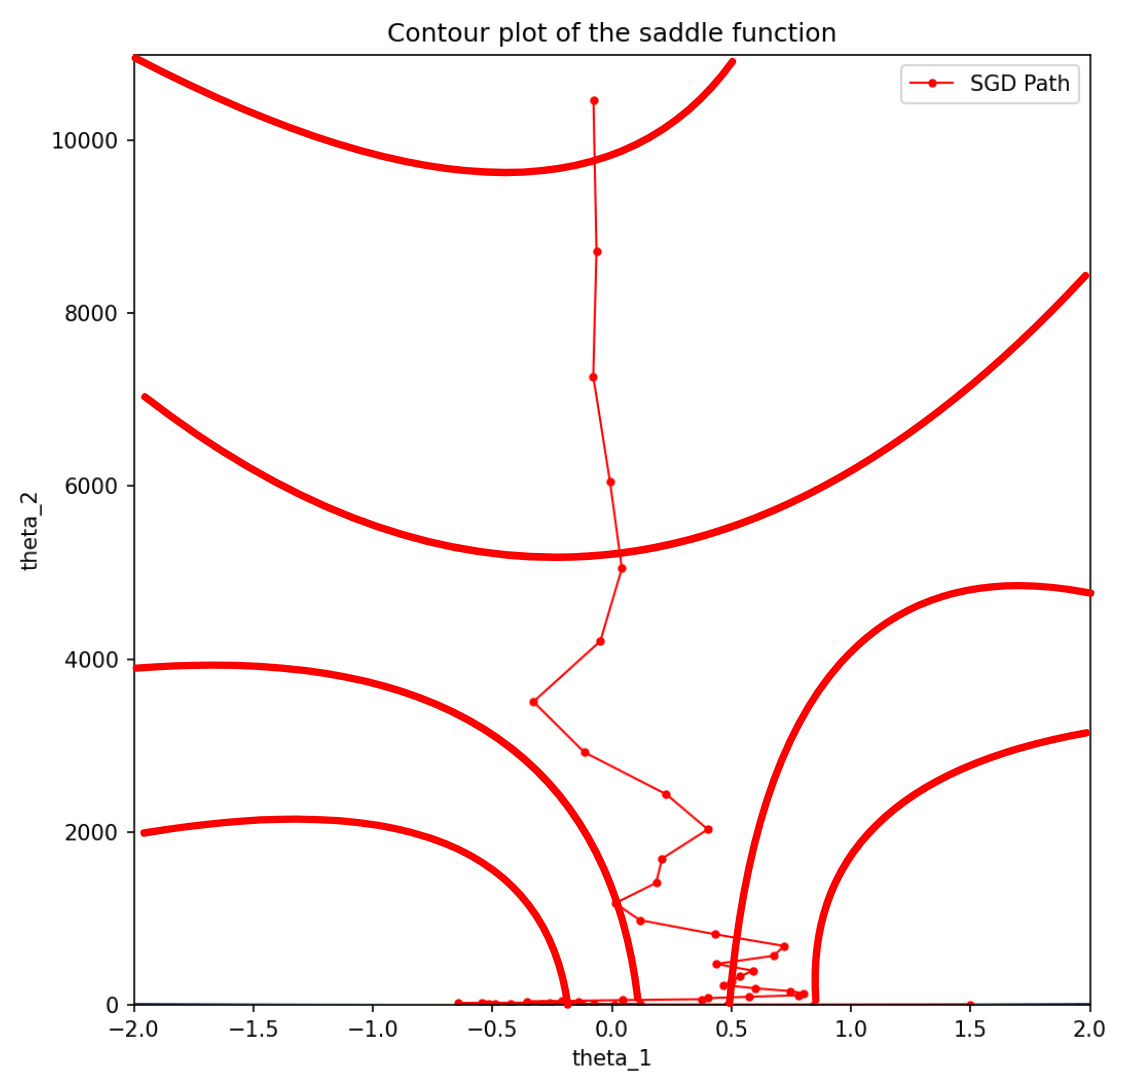
\includegraphics[width=0.5\textwidth]{../lectures/img/saddle-no-momentum-sgd.jpg}
        \caption{在马鞍面上的随机梯度下降}
    \end{figure}

    在上图中, 随机梯度下降由于马鞍面的形状而在一开始缓慢下降, 效率低下。
    于是动量 ($Momentum$) 的概念被引入, 它用于在梯度下降时提供一个由积累而产生的向量值。动量在梯度下降时不断震荡, 徘徊的方向上会不断抵消, 而在稳定缓慢前进的方向上会不断累加, 这个方向上的动量的累加有利于梯度下降更加快地跳出如马鞍面的图形中的鞍点中的区域。
    具体运算步骤如下:

    \begin{figure}[H]
        \centering
        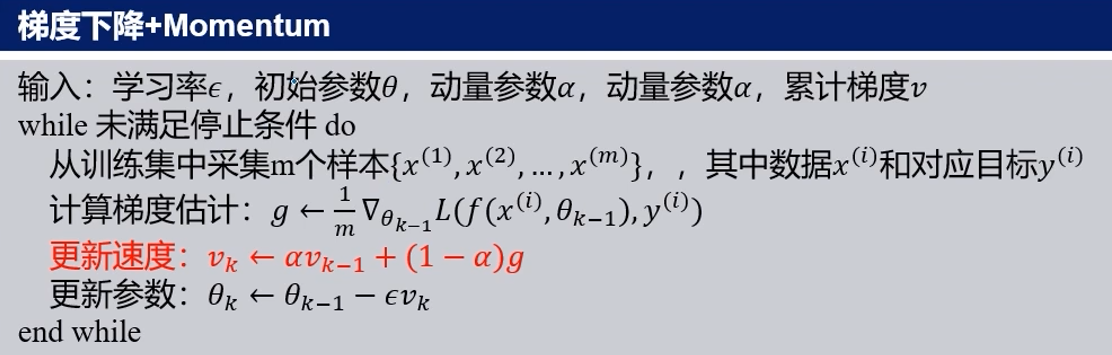
\includegraphics[width=0.7\textwidth]{../lectures/img/gd-with-momentum.jpg}
        \caption{动量梯度下降的步骤}
    \end{figure}

    红色字体的部分展现了动量累积的步骤, 其通过前次动量和当次梯度来累积动量, 其中 \( v \) 是动量, \( \alpha \) 作为动量参数, 在动量更新时起到了保留多少比例的前次动量的作用, 换句话说 \( 1 - \alpha \) 便影响了动量更新的速度。

    \section{$Adagrad$}

    除了调整动量这一方法, 另外一种思路是自适应调整梯度 ($Adagrad$), 
    它根据参数调整学习率, 针对与频繁出现的特征相关的参数执行更小的更新 (即低学习率), \cite{ward2020adagrad}
    针对与不频繁的特征相关的参数执行更大的更新 (即高学习率)。
    一种更加通俗的理解是此算法能做到在震荡的地方步长很小, 而在梯度较小的地方步长变大。\cite{antonakopoulos2022adagrad}
    简要的运算步骤如下:

    \begin{figure}[H]
        \centering
        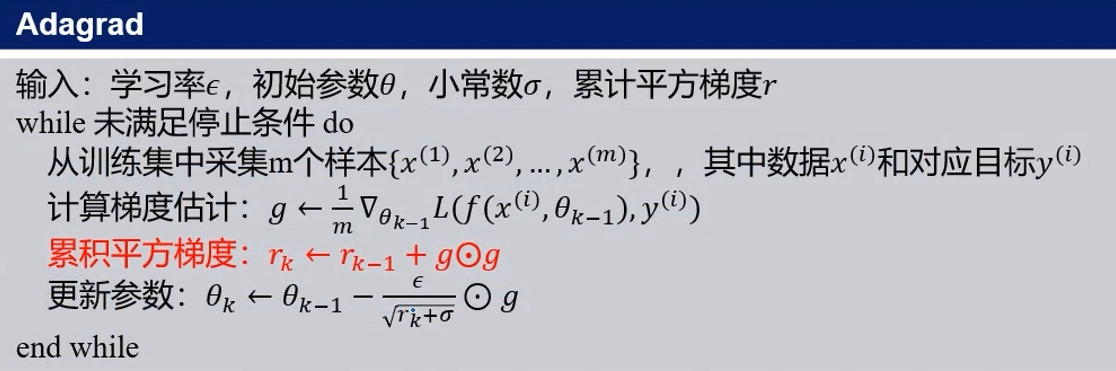
\includegraphics[width=0.7\textwidth]{../lectures/img/adagrad-steps.png}
        \caption{$Adagrad$的运算步骤}
    \end{figure}

    在累积平方梯度时, 如果梯度的平方较大, 那么在下一步更新参数时, 第二项的分母越小, 从而实现梯度的自适应。\cite{duchi2011adaptive}
    特别的是, 在累积平方梯度这一步时, 不是简单地将原来的平方梯度和新的平方梯度相加, 而是在它们之间添加一个比例参数, 
    类似 $Momentum$ 中的 \( \alpha \)\cite{qian1999momentum, sutskever2013importance}, 这便是 \textbf{RMSProp}。


    \section{$Adam$}

    $Adam$ 集合了 $Momentum$ 和 $RMSProp$ 两个的思路, 综合了动量和自适应的优点, 避免了冷启动的问题。\cite{kingma2015adam}
    经验表明, $Adam$ 在实践中表现很好, 和其他适应性学习算法相比也比较不错。
    感谢$bilibili$用户@煮蛋$203$的分享,让我能够在视频里学习到部分Adam的内容:\href{www.bilibili.com/video/BV1YF411n7Dr}{深度学习中的优化器原理}
    
    简要步骤如下:\cite{bilibili2024gradientdescent}

    \begin{figure} [H]
        \centering
        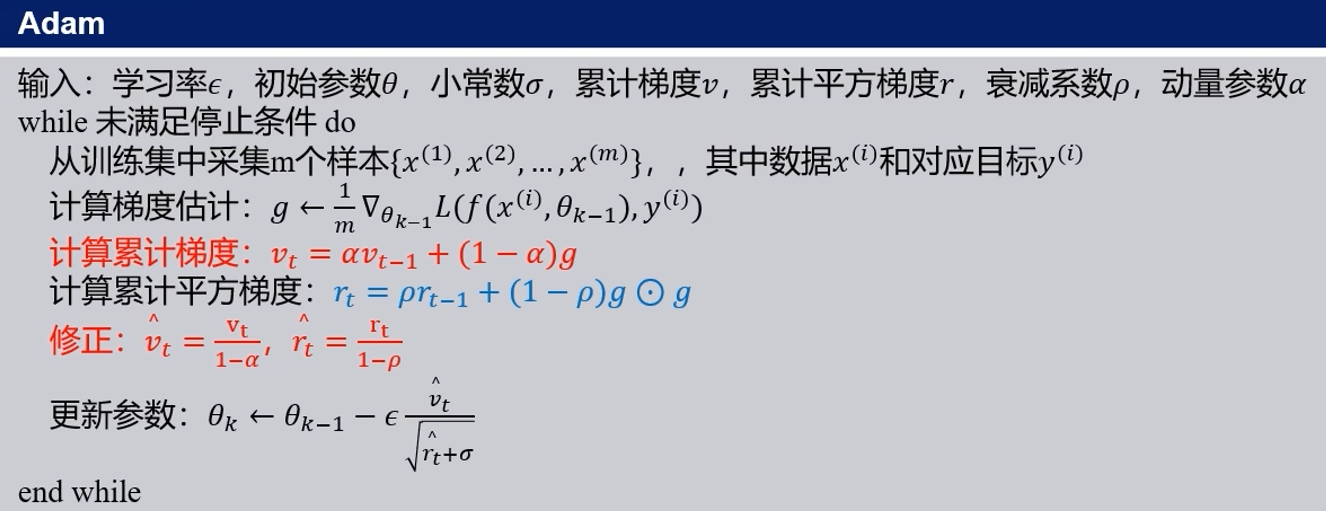
\includegraphics[width=0.7\textwidth]{../lectures/img/adam-steps}
        \caption{$Adam$的运算步骤}
    \end{figure}

    在我的学习中,可以知道其代码实现如下:

    \begin{lstlisting} [language = python, title = {Adam Algorithm}]
    optimizer = optim.Adam(model.parameters(), lr=0.001, betas=(0.9, 0.999))
    \end{lstlisting}

    $Adam$($Adaptive\ Moment\ Estimation$的缩写)是$2014$年对$RMSProp$优化器的更新,
    将其与动量方法的主要特征结合起来。
    在这种优化算法中,使用带有指数衰减的梯度和梯度的二阶矩的运行平均值。
    给定参数 \( w^{(t)} \) 和损失函数 \( L^{(t)} \),其中 \( t \) 表示当前训练迭代(从$0$开始索引),
    Adam的参数更新公式如下:

    \begin{equation}
        m_w^{(t+1)} \leftarrow \beta_1 m_w^{(t)} + (1 - \beta_1) \nabla_w L^{(t)}
    \end{equation}
        
    \begin{equation}
        v_w^{(t+1)} \leftarrow \beta_2 v_w^{(t)} + (1 - \beta_2) (\nabla_w L^{(t)})^2
    \end{equation}
        
    \begin{equation}
        \hat{m}_w = \frac{m_w^{(t+1)}}{1 - \beta_1^t}
    \end{equation}
        
    \begin{equation}
        \hat{v}_w = \frac{v_w^{(t+1)}}{1 - \beta_2^t}
    \end{equation}
        
    \begin{equation}
        w^{(t+1)} \leftarrow w^{(t)} - \eta \frac{\hat{m}_w}{\sqrt{\hat{v}_w} + \epsilon}
    \end{equation}

    其中,\(\epsilon\) 是一个小常数(如 \(10^{-8}\)),用于防止除以$0$,
    \(\beta_1\)(如$0.9$)和 \(\beta_2\)(如$0.999$)分别是梯度和梯度二阶矩的遗忘因子。
    平方和平方根是按元素计算的。

    最初证明$Adam$收敛性的证明并不完整,后续分析表明$Adam$对所有凸目标\cite{reddi2018convergence, rubio2017convergence}都不收敛。
    尽管如此,$Adam$由于其在实践中的强大性能而继续被广泛使用。
    此外,这种算法的深远影响启发了多种新的优化方法,
    如使用$Nesterov$增强梯度的动量优化方案(如$NAdam$和$FASFA$)和解释二阶信息的不同方法(如$Powerpropagation$和$AdaSqrt$)。
    然而,最常用的变种是$AdaMax$\cite{kingma2015adam},它使用无穷范数对$Adam$进行了推广,以及$AMSGrad$,它通过使用过去的最大平方梯度而不是指数平均值来解决$Adam$的收敛问题。
    $AdamW$是一个后来更新,缓解了$Adam$中的权重衰减算法的影响。\cite{ruder2017optimizing}

    \section{梯度下降法在大模型训练中的应用}
    在大模型的训练中,梯度下降法被用于更新模型参数以最小化损失函数。由于大模型参数量巨大,通常使用小批量梯度下降法($Mini-batch\ Gradient\ Descent$)来平衡计算资源和训练效率\cite{hinton2012neural}。

    以$GPT$-$3$为例,其训练过程采用了$Adam$优化器,这是一种基于梯度下降法的自适应学习率优化算法。$Adam$结合了动量和$RMSProp$的优点,能够有效应对大模型训练中的梯度稀疏和梯度消失问题\cite{kingma2015adam}。

    梯度下降法在多个领域中有广泛应用。首先,在机器学习和深度学习中,梯度下降法用于优化模型参数,使得模型对训练数据的误差最小。其次,在经济学和金融学中,梯度下降法用于优化投资组合和风险管理。最后,在工程和物理学中,梯度下降法用于优化复杂系统的控制参数。

    一个实际的应用案例是$Google$的神经机器翻译系统($GNMT$)\cite{zulaika2022students},
    该系统利用梯度下降法来训练其深度神经网络,从而大幅提高翻译的准确性。
    另一个案例是自动驾驶汽车,特斯拉的自动驾驶系统利用梯度下降法不断优化其算法,以实现更安全和更高效的驾驶体验。

    \section{大模型训练中梯度消失与梯度爆炸问题及解决方案}
    在训练深度神经网络时,梯度消失和梯度爆炸是常见问题。
    梯度消失会导致模型参数无法更新,而梯度爆炸则会使参数更新幅度过大。
    为解决这些问题,可以采用批量归一化($Batch\ Normalization$)、残差网络($Residual\ Networks$)
    等技术\cite{he2016deep, ioffe2015batch}。

    \subsection{未来发展方向}
    未来,梯度下降法将在更多领域中发挥重要作用。
    例如,在生物医学领域,梯度下降法将用于优化基因编辑和药物发现。\cite{gupta2021artificial, choudhuri2023recent}
    此外,随着量子计算的发展,梯度下降法可能会结合量子算法,实现更快速和更高效的优化过程。

    随着科技的不断进步,深度学习和大模型正以前所未有的速度改变着我们的世界。
    在这场技术革新中,梯度下降算法如同黑夜中的灯塔,为我们指引了前行的道路。
    从最初的线性回归到如今复杂的神经网络,梯度下降已成为优化算法的中流砥柱。

    每一次的迭代都是对极限的挑战。梯度下降陪伴了我们穿越数据的迷雾,深度学习和大模型必将继续突破现有的边界,探索未知的领域。
    而梯度下降这颗闪耀的明星,必将在每一个前沿领域中持续发挥其光芒。

    \chapter{总述}

    梯度下降法在大模型训练中的应用已成为研究热点。
    $Lemaréchal$($2012$)讨论了柯西梯度法在解决非线性方程中的应用,为梯度下降法奠定了理论基础\cite{lemarechal2012cauchy}。
    $Coursera Staff$($2024$)详细介绍了梯度下降在机器学习中的原理和应用\cite{coursera2024gradientdescent}。
    $Lai$等($2017$)研究了高斯-牛顿法在非线性最小二乘问题中的应用,提供了梯度下降法在实际优化问题中的案例分析\cite{lai2017solving}。
    $Hassan$等($2009$)提出了一种基于准柯西关系的新梯度法,保证了下降性\cite{hassan2009new}。

    $Kingma$和$Ba$($2015$)提出的$Adam$优化器结合了动量和$RMSProp$的优点,显著提升了大模型训练的效率\cite{kingma2015adam}。
    $Yang$和$Wang$($2020$)研究了自适应学习率调度在深度学习模型集成中的应用,展示了梯度下降法的广泛适用性\cite{yang2020auto}。
    $Haji$和$Abdulazeez$($2021$)对基于梯度下降算法的优化技术进行了综述,比较了不同变种的优缺点\cite{haji2021comparison}。
    
    在大模型训练过程中,梯度消失和梯度爆炸是常见问题。
    $He$等($2016$)通过残差网络技术有效解决了梯度消失问题\cite{he2016deep}。
    $Ioffe$和$Szegedy$($2015$)提出的批量归一化方法进一步提升了深度神经网络的训练稳定性\cite{ioffe2015batch}。

% 声明后置部分开始
    \backmatter

% 致谢
    \begin{acknowledgement}
        完成这篇关于梯度下降的文献综述后,我对这一核心算法有了更深的理解和更广泛的视角。
        通过梳理梯度下降的历史发展,我认识到科学家们在算法演进过程中所作出的重要贡献和创新。

        在探索其基本概念和变体时,我进一步理解了不同变体是如何解决原始方法中的一些局限性的。
        文献综述中详细讨论了梯度下降在不同机器学习领域的应用,这让我意识到其广泛的实用性和灵活性。
        尤其是在处理大规模数据集和复杂模型训练方面,梯度下降及其变体显示出了极大的优势。
        通过比较梯度下降与其他优化方法,在不同情况下选择最合适的优化技术。

        同时,我也终于从课堂中对$ReLu$激活函数的陌生变成了熟悉,知道了各种各样的激活函数,如$Sigmoid$、$Tanh$等等,
        也知道了梯度下降法的一些变种,如$SGD$、$Mini-batch$、$Momentum$、$Adagrad$、$Adam$等等。

        这样的过程,不仅提高了我的技术理解,也增强了我在实际应用中解决问题的能力(恰巧这段时间在跟随吴恩达老师的机器学习课程)。
        在撰写该文献综述时,我因此才了解到知网之外的$Google\ Scholar$,了解到了$Sci$-$hub$等获取学术论文的途径,使用了$Zetoro$等软件来管理文献。

        不仅是这样,我还因此开始学习使用 \LaTeX 进行排版,我意识到梯度下降在未来研究的潜力,
        也对我下定决心学习$Pytorch$有了更多的动力。
        显然,在综述的最后,我提到了一些新兴的趋势。
        例如将梯度下降与深度学习框架结合,以及探索无梯度优化方法。
        这些新兴趋势为梯度下降的进一步发展提供了广阔的前景,也激发了我对这一领域继续深入研究的兴趣。

        这次文献综述的撰写不仅是一次知识的积累,也是一次科研方法和写作技巧的提升。
        这将激励我在未来的学术道路上不断探索,追求卓越。

        在此,特别感谢提供$ECNU\ Thesis$模板的作者$Koyamin$:
        \href{https://github.com/Koyamin/ECNUThesis-Undergraduate}{$ECNUThesis-Undergraduate$},
        是他设计的各种接口让我能够展现出更加新颖的排版,向课程报告增添几分色彩,
        同时也因此学习了引用文献的正确方式($bibTex$),也学会了$cls$文件的部分编辑方法,
        还找到了手写公式识别的与$LateX$强关联的网站:\href{https://simpletex.cn/ai/latex_ocr}{LateX\_OCR}。
        我深知自己尚未有完整的能力理解和完整写出这样的文献综述,大部分内容都是借鉴了其他文献,但一切都是值得感恩的,路漫漫。

    \end{acknowledgement}

% 打印参考文献
\PrintReference
% 在命令行中使用 latexmk -xelatex Finalthesis 来编译, 才能正确显示参考文献的编号顺序(否则会出现乱序)

\newpage

\section*{其余参考文献及有所帮助的网址}
% 不会自动编号。标题前不会有数字,不会在目录中生成对应条目(除非手动添加)。

\begin{itemize}
    \item Wikipedia, \textit{Gradient Descent}, \url{https://en.wikipedia.org/wiki/Gradient_descent}, 访问时间:2023年6月9日.
    \item 作者: 知乎用户, \textit{机器学习——从输入到输出}, 2023, \url{https://zhuanlan.zhihu.com/p/580645925}, 访问时间:2023年6月9日.
    \item 深度学习中的优化器原理: \url{https://www.bilibili.com/video/BV1YF411n7Dr}, 访问时间:2023年5月15日.
    \item TensorFlow Playground:\url{https://playground.tensorflow.org}, 访问时间:2023年5月26日.
    \item Fabianp:\url{https://fa.bianp.net/teaching/2018/COMP-652/gradient_descent.html}, 访问时间:2023年5月26日.
    \item LateX\_OCR:\url{https://simpletex.cn/ai/latex_ocr}, 访问时间:2023年5月20日-2023年6月15日.
\end{itemize}

\end{document}